\documentclass[tikz]{standalone}
\usepackage{hepnames}
\usepackage{xpatch}
\makeatletter
\xpatchcmd\@HepConStyle
 {\edef\@upcode{\updefault}}
 {\ifdefined\shapedefault\edef\@upcode{\shapedefault}\else\edef\@upcode{\updefault}\fi}
 {}{}
\makeatother
\usepackage{tikz-feynman}
\makeatletter
\tikzfeynmanset{compat=\tikzfeynman@version@major.\tikzfeynman@version@minor.\tikzfeynman@version@patch}
\makeatother

\begin{document}

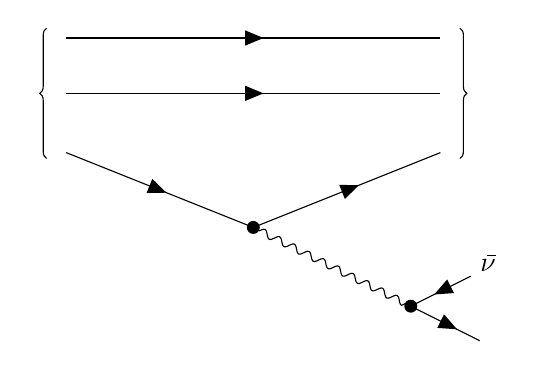
\begin{tikzpicture}
\begin{feynman}
\vertex (d1) {\( \Pdown \)}; 
\vertex[right=5cm of d1] (d2) {\( \Pdown \)}; 
\vertex[below=2em of d1] (u1) {\( \Pup \)}; 
\vertex[right=5cm of u1] (u2) {\( \Pup \)};
\vertex[below=2em of u1] (d3) {\( \Pdown \)}; 
\vertex[right=5cm of d3] (u3) {\( \Pup \)};
\vertex[dot, below right=1cm and 2.5cm of d3] (v1){};
\vertex[dot, below right=1cm and 2cm of v1] (v2){};
\vertex[above right=0.5cm and 1cm of v2] (nu) {\( \APnu_{\Pe} \)};
\vertex[below right=0.5cm and 1cm of v2] (e) {\( \Pelectron \)};
\diagram* { {[edges=fermion]
(d1) -- (d2),  (u1) -- (u2),
(d3) -- (v1) -- (u3), (nu) -- (v2) -- (e)},
(v1) -- [boson, edge label=\( \PWminus \)] (v2)
};
\draw [decoration={brace}, decorate] (d3.south west) -- (d1.north west) node [pos=0.5, left] {\( \Pneutron \)};
\draw [decoration={brace}, decorate] (d2.north east) --  (u3.south east) node [pos=0.5, right] {\( \Pproton \)};
\end{feynman} 
\end{tikzpicture}

\end{document}
